\section{Komponenten}

Im Folgenden werden die einzelnen Komponenten genauer vorgestellt. Die Erläuterungen werden nach Fachbereich gegliedert.

\subsection{Maschinenbau}
\label{sec:komponenten-maschinenbau}

Neben dem Gehäuse, das alle anderen Komponenten zusammenhält und so den Körper von \textit{Silisloth} bildet, werden im Bereich Maschinenbau diverse mechanische Komponenten benötigt. Die Motoren, die Gegenstand der beiden Fachbereiche Maschinenbau und Elektrotechnik sind, werden hierbei der Elektrotechnik zugerechnet.

\subsubsection{Aufhängung}

\begin{figure}
    \centering
    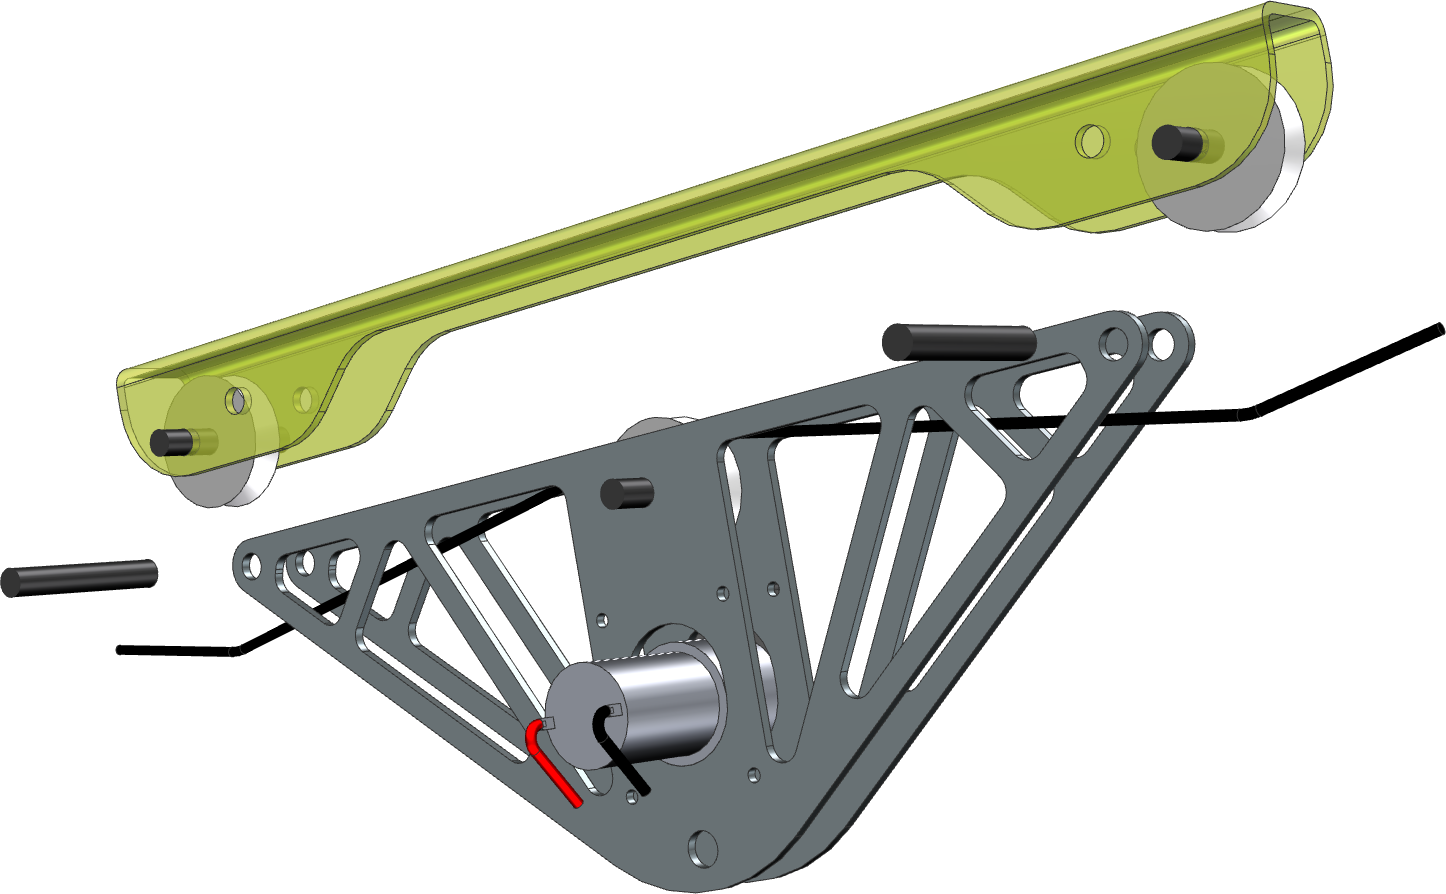
\includegraphics[width=\linewidth]{pics/aufhaengung.png}
    \caption{CAD-Modell der Aufhängung (Explosionsansicht)}
    \label{fig:aufhaengung}
\end{figure}

\begin{description}
\item[Fortbewegung] Die Befestigung und Fortbewegung am Stahlseil wird durch Räder realisiert. Sie bestehen aus Kunststoff, sind 3D gedruckt und haben eine V-förmige Lauffläche. Diese Form führt dazu, dass mehr als nur die Gewichtskraft von \textit{Silisloth} für die Reibung vorhanden ist. Somit kann auch bei einem kleinen Reibungskoeffizienten von $0.13$ die Haftreibung garantiert werden, die eine reibschlüssige Fortbewegung am Seil ermöglicht. (Genauere Berechnungen werden in \appref{app:reibung} angestellt.) Das treibende Rad wird durch einen Getriebemotor, der mit einem Zahnriemen mit dem Rad verbunden ist, angetrieben. Durch den Synchronantrieb kann die momentane Position auf der Längsachse berechnet werden. Der Motor wird über eine Platte auf dem Fachwerk befestigt, damit die Vorspannung des Zahnriemens auch bei sich ändernder Seilsteigung gleich bleibt. Die Platte dient dazu, dass der Zahnriemen ge- und entspannt werden kann. Dies ist bei Zahnriemen nötig, um die geforderte Leistung übertragen zu können. Die Achsen und die Welle sind mit Rillenkugellagern gelagert, um geringe Reibungsverluste zu erzielen.
\item[Gerüst] Die Räder werden an einem Fachwerk-ähnlichen Gerüst befestigt (\imgref{fig:aufhaengung}). Das Fachwerk bietet hohe Biege-Widerstände für wenig Material/Gewicht. Durch das Abstützen am Seil an zwei Orten entsteht ein Biegemoment im Gerüst. Jenes steigt, je weiter die beiden Räder voneinander entfernt sind.
Damit ein Montieren am Seil innerhalb von zwei Minuten möglich ist, kann der Deckel der Aufhängung durch das Entfernen von zwei Stiften geöffnet werden. Das Fachwerk wird aus Aluminium lasergeschnitten und der Deckel 3D gedruckt. Die beiden tragenden Räder werden fertig im Deckel montiert, ebenso ist das Fachwerk mit dem treibenden Rad und dem Getriebemotor fest verbaut. Die beiden Aluminiumplatten des Fachwerks werden durch Distanzhülsen auf der gewünschten Breite gehalten.
\item[Schwingungsdämpfung] Schwingungen in Seilrichtung wird mit Dämpfern entgegengewirkt. Sie werden am Gerüst und am Hauptteil befestigt. Der Hauptteil ist durch einen Bolzen mit dem Gerüst verbunden. Somit liegt der Hauptteil immer waagerecht unter dem Seil. Damit kann garantiert werden, dass der Holzwürfel am gewünschten Ort auf- und abgeladen werden kann. Schwingungen um die Seilachse sollten nicht entstehen können, da sämtliche Kräfte direkt unter dem Seil angreifen. Sollten dennoch solche Schwingungen auftreten, sind sie klein und werden durch die Reibung am Seil gedämpft.
\end{description}

\subsubsection{Seilwinde}

Zur vertikalen Bewegung des Greifers wird eine Seilwinde eingesetzt. Um das Haltemoment des Schrittmotors, welcher die Seiltrommel antreibt, nicht zu überschreiten, wird ein Flaschenzug mit dem Verhältnis 1:2 zur Anwendung kommen. Dies bringt zusätzlich den positiven Nebeneffekt, dass die Last nicht unkontrolliert umherpendeln kann. Die Seiltrommel sowie deren Antrieb sind am Gehäuse angebracht. Als Kraftübertragungsmittel ist ein Zahnriemen vorgesehen, welcher die Möglichkeit bietet, mit den Riemenrädern eine zusätzliche Unter- bzw. Übersetzung zu realisieren.

\subsubsection{Silikongreifer}

Ziel des Silikongreifers ist es, einen Holzwürfel mit einer Kantenlänge von ca. $5cm$ und einem Gewicht von $80g$ zu fassen. Der Greifer ist an einem Seil befestigt, wobei dieses mit der restlichen Vorrichtung verbunden ist. Die Greifvorrichtung verfügt über einen integrierten Luftkanal, welcher durch gezielte Luftzufuhr den eigentlichen Greifmechanismus auslöst. Durch ein Ventil an der Pumpe kann die Luft wieder abgelassen werden, wobei sich die Greifhand langsam öffnet und die Last loslässt. Die Herstellung des Silikongreifers ist in \appref{app:herstellung-silikongreifer} ausführlich beschrieben.

\subsection{Elektrotechnik}
\label{sec:komponenten-elektrotechnik}

Der Bereich Elektrotechnik, der logisch zwischen dem Maschinenbau und der Informatik angesiedelt ist, umfasst im vorliegenden Projekt neben den bereits erwähnten Motoren auch deren Stromversorgung, einen Mikrocontroller und Sensoren. Die Stromversorgung des Mikrocontrollers ist Gegenstand der Informatik, da dieser über das Entwicklerboard gespeist wird.

\subsubsection{Motoren}

Zur Fortbewegung von \textit{Silisloth} und für die Lastaufnahme werden Motoren benötigt. Für das Fahren am Seil kommt ein DC-Motor zum Einsatz, welcher über ein Getriebe \textit{Silisloth} antreibt. Bei der Lastaufnahme werden zwei Motoren benötigt. Ein Motor bringt den Greifarm zur Last, während der zweite Motor den Greifer selbst antreibt. Um die Motoren mit genügend Strom zu versorgen, werden diese über einen Motorentreiber betrieben.

\begin{description}
\item[Motorentreiber] Da \textit{Silisloth} für den Betrieb drei Motoren benötigt, bietet sich das Motorshield von Adafruit \shortcite{motorshield} als Motorentreiber an. Über das Board können 4 Motoren unabhängig voneinander angesteuert werden. Jeder Ausgang liefert bis zu $600mA$ Strom ($1.2A$ Spitze) bei $4.5$ bis $25V$ Spannung (\imgref{fig:motorshield}).
\item[Lastaufnahme] Die Lastaufnahme erfolgt über einen Silikongreifer, der mit Druckluft betrieben wird. Der Greifer wird als Einheit mit einer Miniluftpumpe \shortcite{luftpumpe} zur Last gebracht. Die Luftpumpe wird von einem $6/12V$-DC-Motor angetrieben und befördert ca. $1.8l/min$ bei einer Stromaufnahme von $300mA$ (\imgref{fig:luftpumpe}). Um einen Anhaltspunkt für die Dimensionierung des Motors für die Seilwinde zu erhalten, wurde das Gewicht der Greifeinheit mit einer Last von $1kg$ grosszügig geschätzt. Die Greifeinheit wird über einen Flaschenzug zu ihrem Ziel gebracht. Als erstes wird die Solldistanz von einem Ultraschallsensor ermittelt, dann bringt der Schrittmotor die Einheit zu ihrem Einsatzort. Der Schrittmotor vom Typ Emis E547-52500 \shortcite{schrittmotor} weist ein Haltemoment von $0.25Nm$ auf und wird mit $12V$ und $600mA$ betrieben. Dabei wird eine Umdrehung in 200 Schritte unterteilt, was eine sehr genaue Platzierung der Greifeinheit ermöglicht (\imgref{fig:schrittmotor}).
\item[Antrieb] Die Fortbewegung am Seil wird mit einem DC-Motor realisiert, der \textit{Silisloth} über ein Getriebe antreibt. Da herkömmliche DC-Motoren viel zu hohe Drehzahlen aufweisen und passende Getriebe schwer zu finden oder zu teuer sind, fiel die Wahl auf den Getriebemotor Typ33-125 vom Hersteller Igarashi \shortcite{getriebemotor}, der die hohen Drehzahlen des DC-Motors mit einem integrierten Getriebe untersetzt. Der Igarashi Typ 33-125 wird mit $12V$ und $300mA$ betrieben und liefert $0.3Nm$ Drehmoment bei $38 U/min$ (\imgref{fig:getriebemotor}). 
\end{description}

\begin{figure}
    \centering
    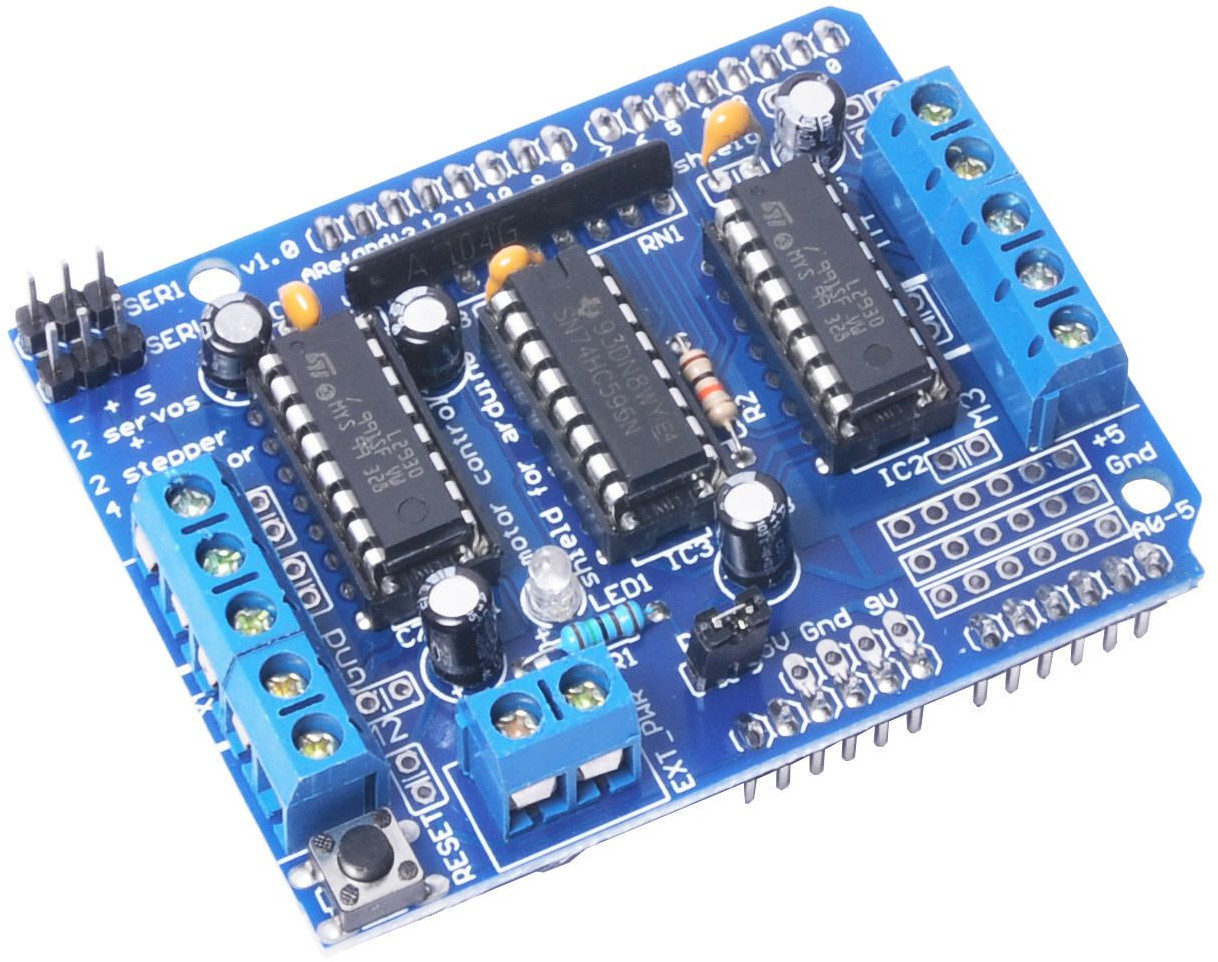
\includegraphics[width=0.5\linewidth]{pics/motorshield.jpg}
    \caption{Motor Shield HP-ASH-L293D}
    \label{fig:motorshield}
\end{figure}

\begin{figure}
    \centering
    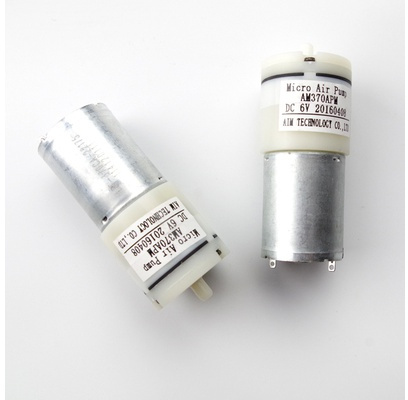
\includegraphics[width=0.5\linewidth]{pics/luftpumpe.jpg}
    \caption{Miniluftpumpe mit Motor}
    \label{fig:luftpumpe}
\end{figure}

\begin{figure}
    \centering
    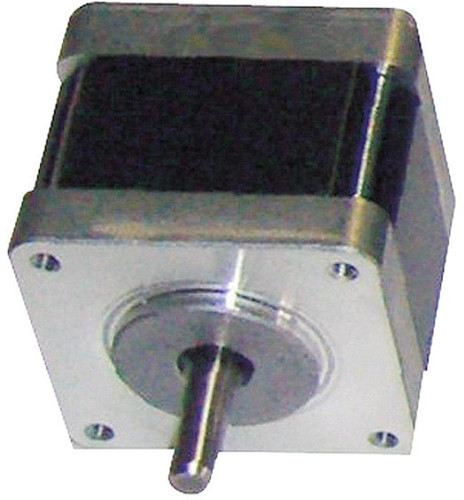
\includegraphics[width=0.5\linewidth]{pics/schrittmotor.jpg}
    \caption{Schrittmotor Emis E547-52500}
    \label{fig:schrittmotor}
\end{figure}

\begin{figure}
    \centering
    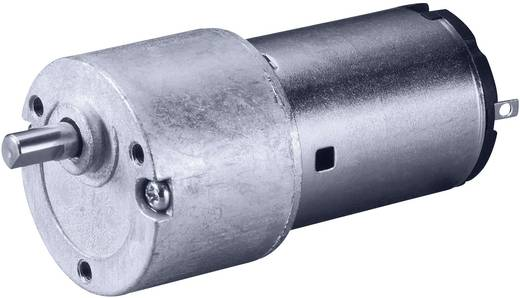
\includegraphics[width=0.5\linewidth]{pics/getriebemotor.jpg}
    \caption{Getriebemotor Igarashi Typ33-125}
    \label{fig:getriebemotor}
\end{figure}

\subsubsection{Ultraschallsensor}

Um zu jedem Zeitpunkt zu wissen, wo sich die aufgenommene Last befindet, werden zwei Ultraschallsensoren des Typs HC-SR04 \shortcite{ultraschallspec} verwendet (\imgref{fig:ultraschallsensor}). Diese sind in der Lage den Abstand zu einem Objekt im Bereich von $3$ bis $400cm$ zu messen. Der eine Sensor misst dabei den Abstand zum Masten am Ende des Seils, während der andere nach unten gerichtet ist und die jeweilige Höhe der Last über dem Boden ermittelt. Der Ultraschallsensor arbeitet mit einer Spannung von $5VDC$, bei einer Stromaufnahme von $<2mA$.

\begin{figure}
    \centering
    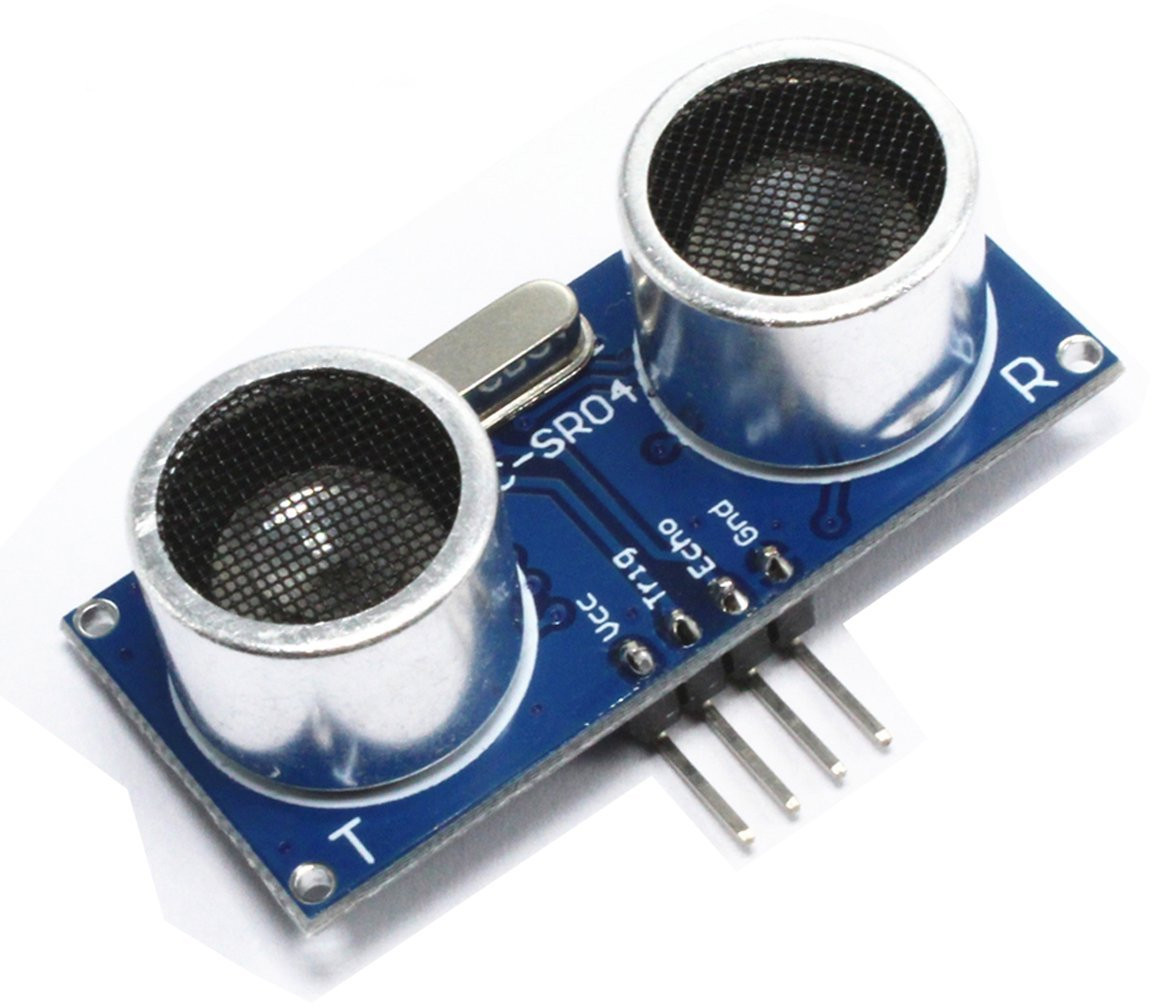
\includegraphics[width=0.5\linewidth]{pics/ultraschallsensor.jpg}
    \caption{Ultraschallsensor HC-SR04}
    \label{fig:ultraschallsensor}
\end{figure}

Eine Messung mit dem HC-SR04 läuft wie folgt ab \shortcite{ultraschallhowto}: Über den Trigger-Anschluss wird eine Messung gestartet. Die fallende Flanke eines min. $10 µs$ langen High-Impulses löst eine Messung aus (\imgref{fig:ultraschall-messung}). Der HC-SR04 sendet daraufhin ein $40 kHz$-Burst-Signal bestehend aus acht Impulsen aus. Danach geht der Echo-Ausgang sofort auf einen High-Pegel und wartet auf das Empfangen eines Echos/Signals. Wird ein solches Echo detektiert, geht der Ausgang wieder auf Low. $20 ms$ nach der Triggerung kann erneut eine Messung gestartet werden. Es können somit $50$ Messungen pro Sekunde durchgeführt werden. Bleibt jedoch ein Echo aus, bleibt der Ausgang für $38 ms$ auf High und signalisiert so eine Fehlmessung.

\begin{figure}
    \centering
    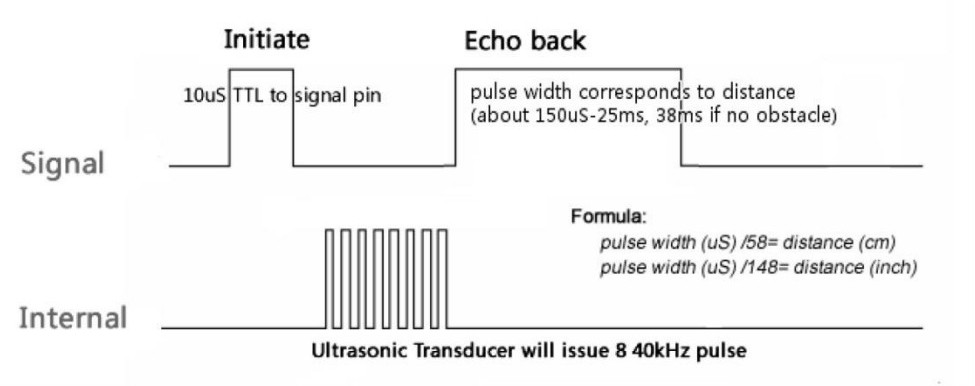
\includegraphics[width=\linewidth]{pics/ultraschall-messung.jpg}
    \caption{Ansteuerung des HC-SR04}
    \label{fig:ultraschall-messung}
\end{figure}

Die gemessene Entfernung ist proportional zur Echo-Puls-Weite und kann wie folgt berechnet werden \shortcite{ultraschallberechnung}:

\begin{equation}
\text{Distanz} = \frac{\text{EchoSignalLänge} * c}{2}, c \approx 340 \frac{m}{s}
\end{equation}

Der Divisor 2 berücksichtigt, dass das Signal den doppelten Weg zurücklegt: zum Objekt hin und wieder zurück. Wird weiter die Schallgeschwindigkeit bei ca. $20\degree C$ verwendet, und die Echo-Signal-Länge in $\mu s$ kann die Formel folgendermassen vereinfacht werden, um die gemessene Distanz in $cm$ zu erhalten.

\begin{equation}
\text{Distanz} = \frac{\text{EchoSignalLänge}}{58}, \text{Distanz in } cm
\end{equation}

Die besten Messergebnisse werden bei einer Reflexion an glatten, ebenen Objekten erzielt. Ab einer Entfernung von über einem Meter muss darauf geachtet werden, dass der Ultraschallsensor möglichst genau auf das zu messende Objekt ausgerichtet wird. Hindernisse, welche sich dann im Sendekegel (ca. $15\degree$) befinden, können die Messung beeinflussen und somit verfälschen. Des Weiteren ist darauf zu achten, dass sich mehrere Ultraschallsensoren, welche nahe beieinander liegen, nicht gegenseitig beeinflussen. Dies und die Messgenauigkeit des Sensors wurden in einem Versuch erprobt (\secref{sec:versuch-ultraschallsensor}).

\subsubsection{Mikrocontroller}
\label{sec:mikrocontroller}

Für die hardwarenahe Programmierung wird das Freedom Development Board FRDM-KL25Z \shortcite{freedomboardspec} von NXP verwendet (\imgref{fig:freedom-board}). Dieses Mikrokontroller-Board ist besonders kostengünstig. Das Herz bildet ein 32-bit ARM Cortex-M0+-Prozessor mit einer Betriebsfrequenz von $48 MHz$. Des Weiteren besitzt es diverse analoge und digitale Peripherie und mehrere UART-Schnittstellen. 

\begin{figure}
    \centering
    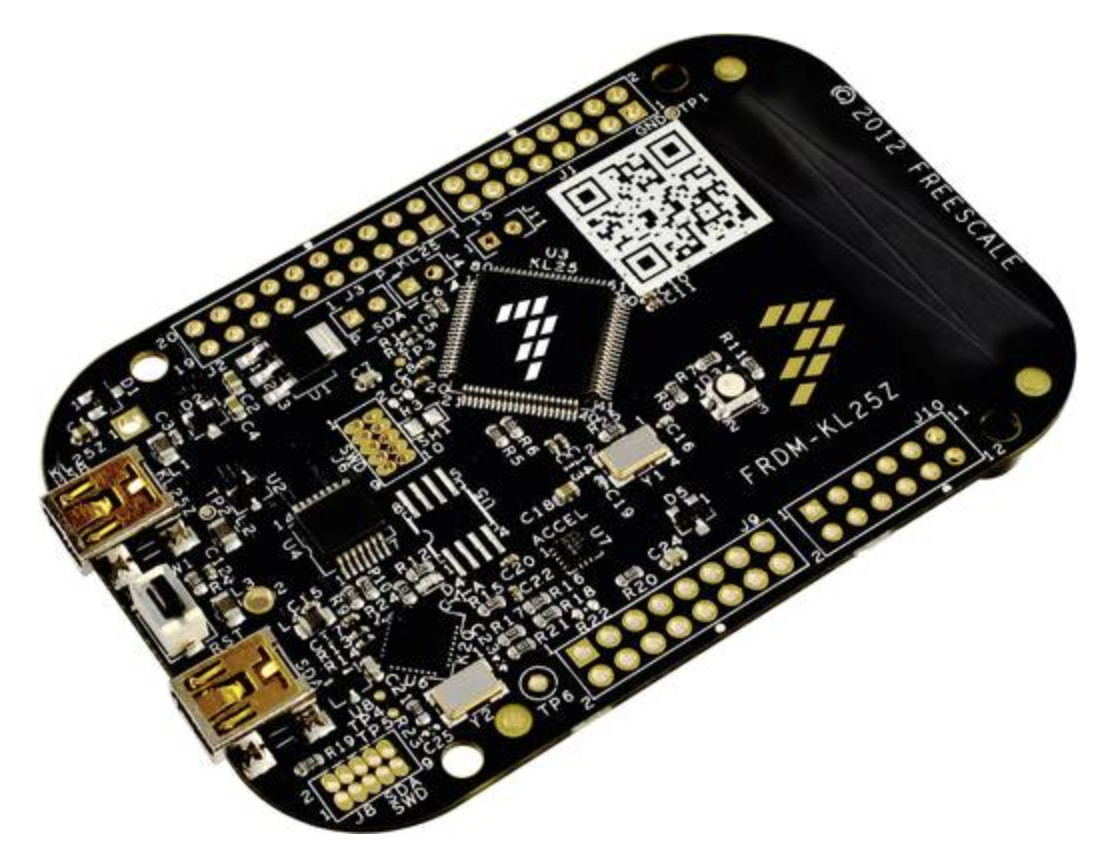
\includegraphics[width=0.5\linewidth]{pics/freedom-board.jpg}
    \caption{Das Freedom-Board FRDM-KL25Z}
    \label{fig:freedom-board}
\end{figure}

Das Freedom-Board wird verwendet um die Motoren des Antriebs und der Lasthebung über Motorentreiber anzusteuern. Zusätzlich kann es auch verwendet werden um die Messungen der Ultraschallsensoren auszuwerten und um das Signal des Endschalters zu empfangen.

Programmiert wird das FRDM-KL25Z über die integrierten Entwicklungsumgebungen (IDE) von Freescale, Kinetis Design Studio oder CodeWarrior. Als Programmiersprache kommt C zum Einsatz. Zusätzlich wird Processor Expert verwendet: ein Tool, welches Embedded-Komponenten verwendet um einfach Quellcode zu generieren.

\subsubsection{Endschalter/Drucktaster}

Um sicherzustellen, dass \textit{Silisloth} am Ende des Seils stoppt und den Antriebsmotor abschaltet, wird ein Mikroendschalter \shortcite{endschalter} verwendet (\imgref{fig:drucktaster}). Dieser wird an der Vorderseite des Geräts angebracht und betätigt, sobald er den Masten am Ende des Seils berührt. Die Signalleitung am Pin des Freedom-Boards wechselt dann von High auf Low und der Antriebsmotor wird angehalten.

\begin{figure}
    \centering
    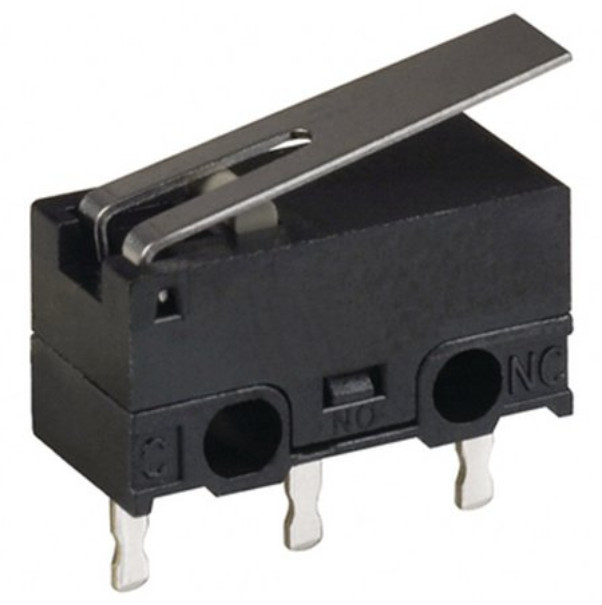
\includegraphics[width=0.5\linewidth]{pics/drucktaster.jpg}
    \caption{Mikroendschalter}
    \label{fig:drucktaster}
\end{figure}

\subsubsection{Stromversorgung}

Damit \textit{Silisloth} seine Aufgabe erfüllen kann, muss es mit Strom versorgt werden. Um einen reibungslosen Ablauf zu garantieren, werden die Informatik- und Elektronikkomponenten von einer separaten Quelle über eine USV mit Powerboost versorgt. Die Motoren werden von einer anderen Quelle gespeist, um bei einem möglichen Spannungsabfall beim Anfahren keinen Neustart der Rechenkomponenten (Mikrocontroller und Entwicklerboard) zu riskieren.

\begin{description}
\item[Akku für Mikrocontroller und Entwicklerboard] Das Entwicklerboard versorgt den Mikrocontroller und den Ultraschallsensor mit Strom. Das Entwicklerboard bezieht die Energie von einem Lithium-Polymer-Akku über eine USV mit Spannungshochsetzer (\secref{sec:usv}). Die einzelnen Komponenten und ihr Energieverbrauch sind in \tblrefplain{tbl:akku1}, aufgelistet\footnote{Das Freedom-Board wird über den Raspi gespiesen. Darum werden hier einige Angaben weggelassen.}.
\item[Akku für Motoren] \textit{Silisloth} benötigt für seinen Betrieb drei Motoren: zwei für die Lastaufnahme und einen für den Antrieb. Die Motoren werden über ein Motorshield von einem Lithium-Polymer-Akku mit Energie versorgt. Der Energieverbrauch der einzelnen Motoren ist in \tblrefplain{tbl:akku2} augelistet.
\item[Berechnung der Akkukapazität] Aus den \tblrefplain{tbl:akku1} und \tblrefplain{tbl:akku2} wird ersichtlich, dass die Rechenkomponenten $630mWh$ und die Motoren $587mWh$ (Angaben gerundet) Energie brauchen. Die Akkukapazitäten werden mit \textit{Formel} \calcrefplain{eq:akku} berechnet. Dabei wird bei den Motoren mit einer Spannung von $12V$ und bei den Rechenkomponenten mit $5V$ gerechnet. Die Berechnungen ergeben eine Mindestkapazität von $126mAh$ für die Rechenkomponenten, und für die Motoren ist ein Akku mit mindestens $49mAh$ Kapazität notwendig.
\end{description}

\begin{equation}
Q=\frac{E}{U}, Q=\text{Ladung in }Ah, E=\text{Energie in }Wh, U=\text{Spannung in }V
\label{eq:akku}
\end{equation}

\begin{table}
\small
\begin{tabularx}{\linewidth}{l|r|r|r|r|r|r}
Komponente & Anzahl & Spannung $[V]$ & Strom $[A]$ & Leistung $[W]$ & Laufzeit $[s]$ & Energie $[Wh]$ \\
\hline
Raspi mit Kamera & $1$ & $5$ & $2.5$ & $12.5$ & $180$ & $0.625$ \\
\hline
Freedom-Board & $1$ & $5$ & - & - & - & - \\
\hline
Ultraschallensor & $2$ & $5$ & $0.015$ & $0.075$ & $180$ & $0.00375$ \\
\hline
Total & $4$ & $5$ & $2.515$ & $12.575$ & $360$ & $0.62875$ \\
\end{tabularx}
\caption{Berechnung der Akku-Kapazität für die Rechenkomponenten\label{tbl:akku1}}
\end{table}

\begin{table}
\small
\begin{tabularx}{\linewidth}{l|r|r|r|r|r|r}
Komponente & Anzahl & Spannung $[V]$ & Strom $[A]$ & Leistung $[W]$ & Laufzeit $[s]$ & Energie $[Wh]$ \\
Getriebemotor & $1$ & $12$ & $0.38$ & $4.56$ & $180$ & $0.228$ \\
\hline
Schrittmotor & $1$ & $12$ & $0.6$ & $7.2$ & $150$ & $0.299$ \\
\hline
Mini-Luftpumpe & $1$ & $12$ & $0.3$ & $3.6$ & $60$ & $0.06$ \\
\hline
Total & $3$ & $12$ & $1.28$ & $15.36$ & $490$ & $0.58$ \\
\end{tabularx}
\caption{Berechnung der Akku-Kapazität für die Motoren und die Luftpumpe\label{tbl:akku2}}
\end{table}

\subsection{Informatik}
\label{sec:komponenten-informatik}

In der Informatik ist das Entwicklerboard die zentrale Komponente. Dieses schränkt nicht nur die Wahl der Hard- und Softwarekomponenten (Kamera, Betriebssystem, Programmierungebung) ein, sondern bedarf auch einer bestimmten Stromversorgung. Das Netzwerk ist dabei von besonderer Bedeutung. Da es sich hierbei nicht um eine eigentliche Komponente, sondern um ein geräteübergreifendes Kommunikationssystem handelt, wird dieses unter \textit{Schnittstellen} (\secref{sec:netzwerk}) beschrieben.

\subsubsection{Entwicklerboard}

Als Entwicklerboard wird der Raspberry Pi Model B Version 3 (fortan als \textit{Raspi} bezeichnet) verwendet. Mit seiner 4-Core-ARM-CPU mit einer Taktrate von $1200 MHz$ und $1 GB$ RAM \shortcite{raspispec} bietet dieses Entwicklerboard genügend Leistung für rechen- und speicherintensive Aufgaben wie Bildverarbeitung und bleibt dank der Multicore-CPU dennoch auch bei hoher Last ansprechbar. Dieses Entwicklerboard bietet ein integriertes WiFi-Interface, womit das Konnektivitätsproblem gelöst wird (\secref{sec:netzwerk}).

\begin{figure}
    \centering
    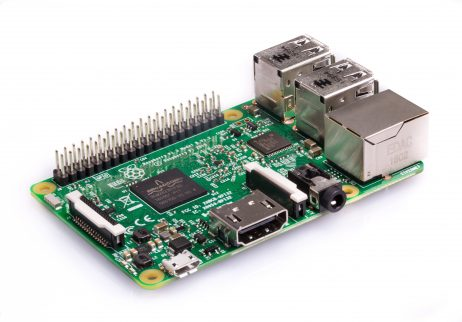
\includegraphics[width=0.5\linewidth]{pics/raspi.jpg}
    \caption{Raspberry Pi Model B Version 3}
    \label{fig:raspi}
\end{figure}

Es gibt auch andere Entwicklerboards, die ähnliche oder gar noch höhere Leistungsmerkmale aufweisen, diese sind aber wesentlich teurer als der Raspi. Die OpenCV-Library benötigt nicht nur viel Leistung bei der Ausführung, sondern auch viel persistenten Speicherplatz (ca. $2 GB$). Mit austauschbaren SD-Karten kann dieses Problem sehr gut gelöst werden. Es ist auch möglich, dasselbe Entwicklerboard mit verschiedenen Konfigurationen zu testen, indem einfach die SD-Karte ausgetauscht wird. Zum Einsatz kommen soll eine SD-Karte mit $32 GB$ Speicherkapazität. Dies genügt nicht nur für Betriebssystem mit den verschiedenen Entwicklertools (Python, OpenCV), sondern auch zur Speicherung verschiedenster Testdaten, die bei den Tests mit der Kamera und Bildverarbeitung entstehen (v.a. Video- und Bilddateien). Zudem bietet der Raspi ein Kamerainterface, womit die Raspi-Cam (\secref{sec:kamera}) einfach angeschlossen und in Betrieb genommen werden kann.

\subsubsection{Betriebssystem}

Die Wahl des Betriebssystems ist stark durch die Auswahl des Entwicklerboards eingeschränkt. Das Flaggschiff unter den Raspi-Betriebssystemen ist Raspbian -- ein Debian-Derivat speziell für den Raspi. Debian zeichnet sich durch hohe Stabilität und weite Verbreitung (im Linux-Umfeld) aus und verfügt über $35000$ Softwarepakete \shortcite{raspbian-faq} mit entsprechender Dokumentation dazu\footnote{Tatsächlich umfasst Raspbian gegenwärtig über $37198$ Softwarepakete (Stand 08.12.2017)}.

Raspbian gibt es in zwei Varianten: Lite und Desktop. Zwar wäre eine grafische Oberfläche bei Experimenten mit der Bildverarbeitung sehr hilfreich, diese konsumiert aber sehr viele Ressourcen, was für den praktischen Betrieb von Nachteil ist. Aus diesem Grund soll Raspbian Lite verwendet werden.


\subsubsection{Programmiersprache}

Als Programmiersprache auf dem Raspi wird Python 3.5 verwendet \shortcite{python-brochure}. Python hat den Vorteil, dass viele mächtige Bibliotheken dafür existieren. Mit diesen Bibliotheken können wichtige Kernfunktionen, wie zum Beispiel die Zielfelderkennung, sehr einfach implementiert werden. Für die Bildverarbeitung wird die Bibliothek OpenCV verwendet \shortcite{opencv-about}. OpenCV bietet bereits ein Python-Interface an, womit die Bildverarbeitung viel einfacher möglich ist als mit anderen Sprachen. Des Weiteren ist der Python-Quellcode leicht lesbar und kann direkt auf dem Raspi editiert und ausgeführt werden. Zur Entwicklung genügt ein einfacher Texteditor. Da Python eine interpretierte Sprache ist, fällt der Kompilierungsschritt weg, was schnelle Entwicklungs- und Testzyklen erlaubt. Aufgrund der vielen genannten Vorteile wird auf dem Raspi die Programmiersprache Python verwendet.

\subsubsection{Kamera}
\label{sec:kamera}

Für die Erkennung der Last und des Zielfelds wird eine Kamera benötigt. Mit dieser Kamera ist es möglich, auf dem Raspi Bilder und Videos zu machen. Diese Aufnahmen werden analysiert um die Last und das Zielfeld zu erkennen. Für den Raspi existiert bereits ein geeignetes Kameramodul: das \textit{Raspberry Camera Module V2} \shortcite{raspi-cam} 

\begin{figure}
    \centering
    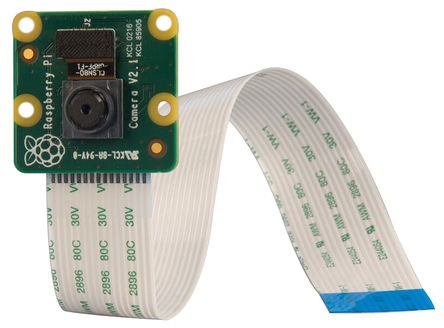
\includegraphics[width=0.5\linewidth]{pics/raspi-cam.jpg}
    \caption{Das Raspberry Pi Camera Module V2}
    \label{fig:raspi-cam}
\end{figure}


Die Kamera eignet sich besonders dadurch, dass auf dem Raspi bereits ein direkter Anschluss vorhanden ist. Diese wird über ein Flachbandkabel (\imgref{fig:raspi-cam}) direkt mit der passenden Schnittstelle mit dem Raspi verbunden. Die Kamera ist bereits für unter CHF 30.- erhältlich \footnote{\url{https://www.pi-shop.ch/raspberry-pi-kamera-module-v2}}. Die Kamera hat $8$ Megapixel und eine maximale Auflösung von $3280 \times 2464$ Pixel für Fotos. Bei Videos sind je nach Auflösung mehr oder weniger Bilder pro Sekunde möglich. Bei $1920 \times 1080$ Pixel sind $30$ Bilder pro Sekunde möglich. Reduziert man die Auflösung auf $1280 \times 720$ Pixel, sind es bereits $60$ Bilder pro Sekunde.

Mittels dieses Kameramoduls wurden in der Verifizierungsphase Aufnahmen gemacht um zu überprüfen, ob diese Kamera geeignet ist. \imgrefplain{fig:foto-zielfeld} zeigt ein Bild des Zielfelds, welches vom Raspi über das Kameramodul gemacht wurde.

\begin{figure}
    \begin{subfigure}{0.5\textwidth}
        \centering
        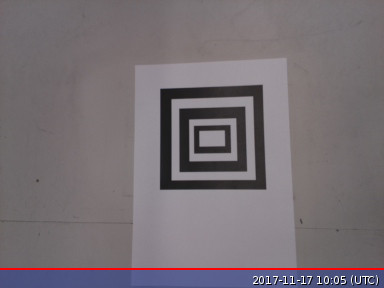
\includegraphics[width=0.9\linewidth]{pics/foto-zielfeld.jpg}
        \caption{Ein Foto vom Zielfeld}
        \label{fig:foto-zielfeld}
    \end{subfigure}
    \begin{subfigure}{0.5\textwidth}
        \centering
        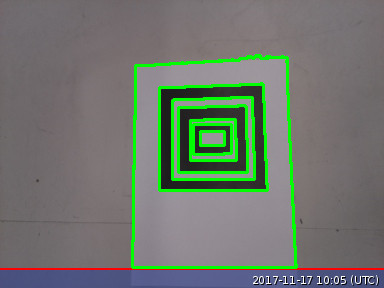
\includegraphics[width=0.9\linewidth]{pics/foto-zielfeld-konturen.jpg}
        \caption{Das Zielfeld mit erkannten Konturen}
        \label{fig:foto-zielfeld-konturen}
    \end{subfigure}
    \caption{Das fotografierte Zielfeld (links) mit erkannten Konturen (rechts)}
\end{figure}

Da in der Aufnahme das Zielfeld gut erkennbar und die Kamera bereits sehr günstig erhältlich ist, wird für das Projekt die offizielle Raspberry-Kamera verwendet werden.

\subsubsection{Bildverarbeitung}

Für die Erkennung des Lastwürfels und des Zielfelds wird die freie Library OpenCV \shortcite{opencv-about} verwendet. OpenCV wurde unter anderem für die Programmiersprache Python geschrieben, durch welche \textit{Silisloth} gesteuert wird. Um OpenCV verwenden zu können, muss zuerst die aktuelle Version auf den Raspi heruntergeladen werden. Anschliessend wird OpenCV auf dem Raspi kompiliert und installiert. Aufgrund der enormen funktionalen Möglichkeiten, die OpenCV bietet, entsteht nach dem Kompilieren ein Buildverzeichnis von über $2 GB$. Nachdem die Installation erfolgreich durchgeführt worden war, wurde ein erster Test zur Erkennung des Zielfelds über OpenCV unternommen. Dazu wurde ein Bild verwendet, welches bereits bei der Verifizierung des Kameramoduls entstanden ist und dadurch direkt über den Raspi und das dazugehörige Kameramodul gemacht wurde. 

Als erstes wird das Bild mit OpenCV geladen. Anschliessend wird das komplette Bild verarbeitet, wobei per OpenCV alle Konturen markiert werden, die weiss oder schwarz sind. Das komplette Python-Skript, welches die Bilderkennung durchführt, ist gerade einmal 14 Zeilen lang. Die Konturenerkennung ist nur deshalb mit so wenigen Zeilen möglich, da das Finden und Zeichnen dieser Konturen über die OpenCV-Library erfolgt. Das Ergebnis der Zielfelderkennung ist auf \imgrefplain{fig:foto-zielfeld-konturen} zu sehen.

\subsubsection{Stromversorgung}
\label{sec:usv}

Wie für das Netzwerk gilt auch bei der Stromversorung, dass sie in der Entwicklungsphase per Kabel erfolgen kann, diese Möglichkeit aber im Test- und Wettbewerbsbetrieb nicht mehr besteht. Darum muss der Raspi über einen Akku betrieben werden. Ein Raspi bezieht je nach Rechenlast (und angeschlossenen Peripheriegeräten) zwischen $1A$ und $2.5A$ Strom bei einer Spannung von $5V$. Ein Akku mit $3000mAh$ sollte bis zu $72$ Minuten (\calcref{eq:betriebsdauer}) und somit bei Weitem für die Wettbewerbssituation ausreichen, bei der \textit{Silisloth} während nur weniger Minuten vom Stromnetz getrennt werden muss.

\begin{equation}
    t = \frac{3000mAh}{2.5A} = 1200 \frac{mAh}{A} = 1.2h = 72\text{min}
    \label{eq:betriebsdauer}
\end{equation}

Damit der Raspi während der Einrichtungsphase nicht neu gestartet werden muss, was aufgrund sporadisch durchzuführender Startup-Tasks (Dateisystem-Integritätsprüfung, Aktualisierung des Dateiindexes etc.\footnote{Derlei Aufgaben könnten natürlich deaktiviert werden, was jedoch zeitaufwändig ist und zu Fehlern führen könnte: Schliesslich gibt es einen Grund dafür, warum gewisse Prüfungen beim Aufstarten gelegentlich ausgeführt werden.}) oder unverhofft auftretenden Probleme zu Verzögerungen führen kann, soll eine USV (unterbruchsfreie Stromversorgung) zum Einsatz kommen (\imgref{fig:usv}). Diese verfügt über drei Anschlüsse:

\begin{figure}
    \centering
    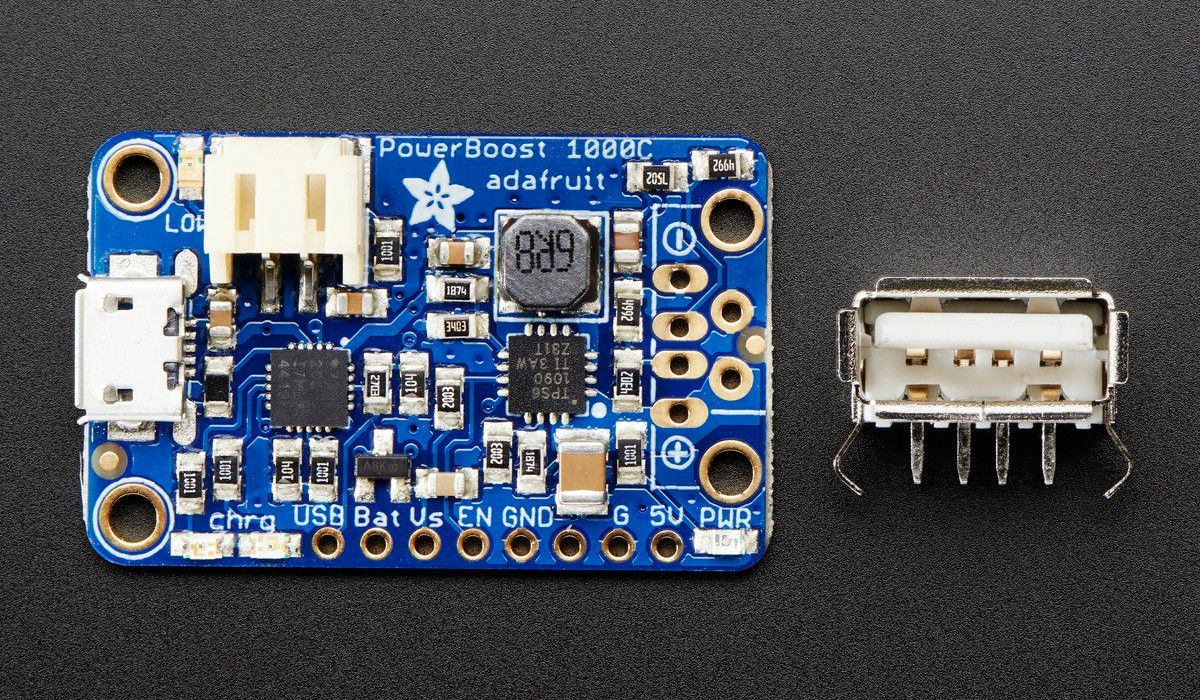
\includegraphics[width=0.5\linewidth]{pics/usv.jpg}
    \caption{USV Adafruit PowerBoost 1000C}
    \label{fig:usv}
\end{figure}

\begin{enumerate}
\item USB-Mini B (links): Hier wird die USV über ein Netzteil an das Stromnetz angeschlossen.
\item Akku (oben): Hier wird ein Lithium-Polymer-Akku angeschlossen.
\item USB-Anschluss (rechts, noch nicht aufgelötet): Hier wird der Raspi per Kabel angeschlossen.
\end{enumerate}

Die USV funktionierte zunächst nicht, da ein Netzteil mit einer Stromstärke von $2.5A$ verwendet wurde. Zwar wurde der Akku geladen und entladen, beim Ein- und Ausstecken des Netzteils kam es aber jeweils zu einem Neustart des Raspis. Mit einem Netzteil der Stromstärke $1A$ funktionierte die USV tadellos, sprich unterbrechungsfrei.

\subsubsection{Smartphone-App}
Mit einer Smartphone-App wird eine Verbindung zwischen Smartphone und \textit{Silisloth} hergestellt. Dies geschieht über eine WiFi-Verbindung. Um \textit{Silisloth} zu starten, wird eine Taste auf der App gedrückt. Ab jetzt läuft \textit{Silisloth} völlig autonom. Sobald \textit{Silisloth} dieses Startsignal empfangen hat, wird der Antrieb gestartet und der Lastwürfel gesucht. Wenn der Lastwürfel aufgenommen wurde, beginnt die App die aktuellen x- und z-Koordinaten des Würfels anzuzeigen. Durch eine konstante TCP/IP-Ver\-bin\-dung zwischen Smartphone und \textit{Silisloth} werden diese Koordinaten laufend aktualisiert. Dies geschieht so lange, bis die Last wieder abgesetzt wurde. Auf \imgrefplain{fig:app} ist das User-Interface der Smartphone-App schematisch dargestellt:

\begin{figure}
    \centering
    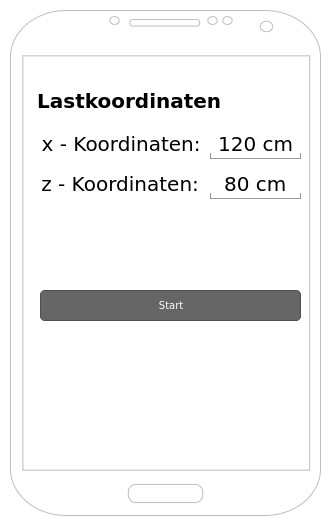
\includegraphics[width=0.5\linewidth]{pics/app.jpg}
    \caption{Das User-Interface der Smartphone-App (schematisch)}
    \label{fig:app}
\end{figure}

\subsection{Alternativen}
\label{sec:komponenten-alternativen}

Wie im Risikomamagement erörtert wird (\secref{sec:risikomanagement}), stellen einige Komponenten bzw. die fehlende Erfahrungen damit eine Gefährdung des Projektziels dar. Für diese Komponenten sollen darum Alternativen gefunden werden, auf die im Problemfall zurückgegriffen werden kann.

\subsubsection{Mikrocontroller: Arduino/Freedom-Board}

Im Bereich Embedded Systems wurden zwei Mikrocontroller untersucht und verglichen: den Arduino Uno Rev3 \shortcite{arduino-uno}, der auf \imgrefplain{fig:arduino} abgebildet ist, und das FRDM-KL25Z Freedom-Board von NXP. Arduino ist im Einsteiger- und Hobbybereich sehr beliebt und weit verbreitet. Mit dem Freedom-Board hingegen wird an der HSLU ‒ Technik \& Architektur gearbeitet. Beide Varianten haben Vor- und Nachteile (\tblref{tbl:microcontroller-vergleich}).

\begin{table}
\begin{tabularx}{\textwidth}{l|X|X|}
& \textsc{Arduino Uno Rev3} & \textsc{FRDM-KL25Z} \\
\hline
Vorteile & 
\begin{itemizecell}{5.8cm}
viele Codebeispiele und fertig implementierte Libraries online vorhanden \\
grosse, hilfreiche Community und Online-Blogs \\
vereinfachte Programmierumgebung
\end{itemizecell}
&
\begin{itemizecell}{5.8cm}
Lerneffekt hoch \\
übersichtliche Programmierumgebung \\
Debugger vorhanden \\
Unterstützung durch HSLU-Dozenten vor Ort möglich
\end{itemizecell} \\
\hline
Nachteile &
\begin{itemizecell}{5.8cm}
online gefundener Code muss auf seine Funktionalität überprüft werden \\
kein Debugger vorhanden \\
Lerneffekt eher gering \\
begrenzte Übersichtlichkeit in der Programmierumgebung 
\end{itemizecell}
&
\begin{itemizecell}{5.8cm}
lange Einarbeitungszeit in Programmierumgebung nötig \\
weniger Codebeispiele online vorhanden \\
geringers Know-How vorhanden
\end{itemizecell} \\
\hline
\end{tabularx}
\caption{Vor- und Nachteile des Arduino Uno Rev3 gegenüber dem FRDM-KL25Z\label{tbl:microcontroller-vergleich}}
\end{table}

Was die Performance und die nötige Peripherie betrifft, sind sich die beiden Mikrocontroller-Boards ebenbürtig. Die Aufgabenstellung ist sicherlich mit beiden zu bewältigen. Wie bereits erwähnt (\secref{sec:mikrocontroller}) ist die Wahl auf das FRDM-KL25Z Freedom-Board gefallen. Da davon auszugehen ist, dass relativ viel Code geschrieben werden muss um die Motoren anzusteuern und um mit dem Raspi zu kommunizieren, wird die Übersichtlichkeit in der Programmierumgebung hoch gewichtet. Die lange Einarbeitungszeit und das fehlende Know-How wird im Austausch gegen den hohen Lerneffekt in Kauf genommen.

\begin{figure}
    \centering
    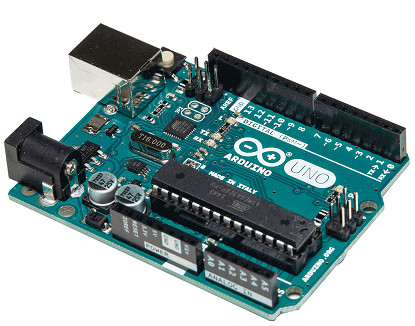
\includegraphics[width=0.5\linewidth]{pics/arduino.jpg}
    \caption{Arduino Uno Rev3}
    \label{fig:arduino}
\end{figure}

Sollten während der Umsetzung unerwartet Probleme mit dem Freedom-Board auftreten, welche nicht fristgerecht gelöst werden können, wird die Option freigehalten auf den Arduino zu wechseln. Der Wechsel auf den Arduino UNO oder Arduino Mega 2560 R3 kann problemlos garantiert werden, da alle verwendeten Komponenten auch zum Arduino kompatibel sind.

\subsubsection{Greifmechanismus: Silikongreifer/Elektromagnet}

Für den Greifmechanismus musste die Entscheidung zwischen dem selbstgebauten Silikongreifer und einem gekauften Elektromagneten getroffen werden. Der Silikongreifer besteht aus zwei verschiedenen Komponenten, welche flüssig zusammengeführt wurden und in einer vorgedruckten Giessform aushärten konnten. Beim Elektromagneten kann eine Kraft von bis zu 300 Newton aufgenommen werden, was für die aufzunehmende Last mehr als ausreichend ist. Eine Gegenüberstellung von Silikongreifer und Elektromagnet (\tblref{tbl:silikongreifer-elektromagnet}) ergab, dass der Silikongreifer die besser geeignete Variante ist, der Elektromagnet aber eine verlässliche Alternative dazu darstellt.

\begin{table}
\begin{tabularx}{\linewidth}{l|X|X|}
& \textsc{Silikongreifer} & \textsc{Elektromagnet} \\
\hline
Vorteile &
\begin{itemizecell}{5.8cm}
kleine Positionierungsfehler können aufgrund der grossen Spannweite noch während des Greifvorgangs ausgeglichen werden \\
nicht-magnetische Last kann angehoben werden \\
optisch interessant \\
innovativ
\end{itemizecell}
&
\begin{itemizecell}{5.8cm}
einfach in der Anwendung \\ 
weniger Funktionsschritte \\
\end{itemizecell}
\\
\hline
Nachteile &
\begin{itemizecell}{5.8cm}
viele und aufwändige Herstellungsschritte \\
braucht eine gesteuerte Luftversorgung 
\end{itemizecell}
& 
\begin{itemizecell}{5.8cm}
Position beim Heben muss viel genauer sein als beim Silikongreifer, da der magnetische Teil der Last sehr klein ist \\
nur magnetische Teile können angehoben werden
\end{itemizecell}
\\
\hline
\end{tabularx}
\caption{Vor- und Nachteile des Silikongreifers gegenüber dem Elektromagneten}
\label{tbl:silikongreifer-elektromagnet}
\end{table}

Sollten in der Umsetzung unerwartete Probleme mit dem Silikongreifer auftreten, welche nicht fristgerecht gelöst werden können, wird die Option freigehalten auf den Elektromagneten zu wechseln. Der Wechsel auf den Elektromagneten kann problemlos garantiert werden, denn dieser wurde in einem Versuch (siehe \appref{app:elektromagnet}) erfolgreich getestet.

\subsection{Schnittstellen}

Für die volle Funktionalität des Systems muss dieses in Komponenten aufgeteilt werden. Diese Komponenten erfüllen Teilaufgaben um die Gesamtaufgabe zu lösen. Dabei kommunizieren die Komponenten über Schnittstellen miteinander. \imgrefplain{fig:hardware-architektur} zeigt, wie die einzelnen Komponenten miteinander verbunden sind.

\begin{figure}
    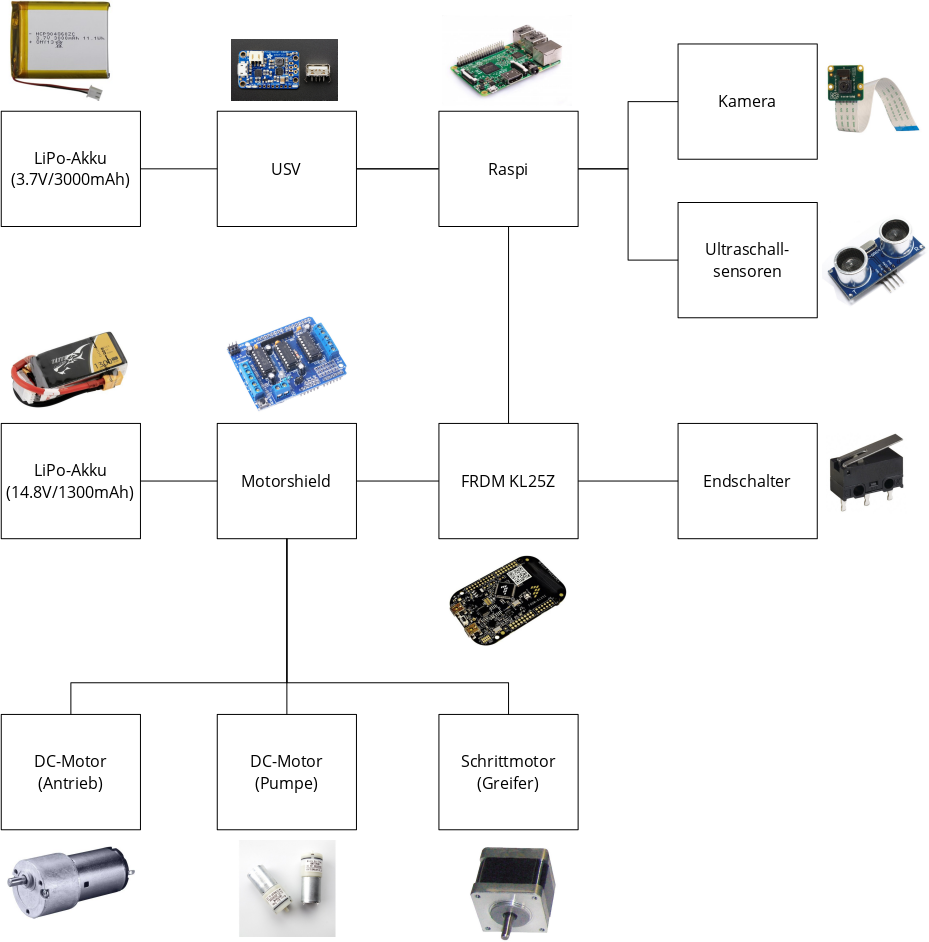
\includegraphics[width=\linewidth]{graphs/schnittstellen.png}
    \caption{Die Hardware-Architektur: Komponenten und Schnittstellen}
    \label{fig:hardware-architektur}
\end{figure}

\subsubsection{Entwicklerboard/Mikrocontroller}

Die Hardware-Architektur zeigt, dass die Steuerung des Systems über den Raspi erfolgt. Dieses kommuniziert mit dem Freedom-Board KL25Z, um die Antriebsmotoren, den Motor zur Anhebung der Last und die Mini-Luftpumpen für den Silikongreifer anzusteuern. Dabei erfolgt die Verbindung des Raspi  mit dem Freedom-Board über eine USB-CDC-Schnittstelle\footnote{Wie diese Verbindung hergestellt wird, ist in einem Blogeintrag \shortcite{usb-cdc} hervorrangend erklärt.}, welche gleichzeitig das Mikrokontrollerboard mit Strom versorgt. USB CDC implementiert ein «Serial over USB»-Protokoll und ist ein einfacher und eleganter Weg um die Kommunikation der beiden Boards sicherzustellen.

Das übertragene Signal vom Raspi zum Freedom-Board enthält die Antriebsgeschwindigkeit und die Antriebsrichtung. Das Freedom-Board leitet diese Befehle an die Motoren weiter. Um die Höhe der Last zu erfahren, kann die aktuelle Position des Schrittmotors, der zum Anheben der Last benötigt wird, abgefragt werden.

Eine weitere Schnittstelle besteht zwischen dem Raspi und dem Smartphone. Die Kommunikation erfolgt hierbei über ein Wireless-Netzwerk. Vom Smartphone wird das Startsignal an den Raspi gesendet. In die Gegenrichtung werden fortlaufend die Koordinaten der aufgenommenen Last an das Smartphone gesendet. Somit erfährt der Anwender jederzeit die Position der Last über sein Smartphone mit der entsprechenden App.

Der Raspi selbst enthält neben der Steuerungslogik auch die Bildverarbeitung. Dazu wird mit einer angeschlossenen Kamera fortlaufend ein Bild des Untergrunds gemacht. Dadurch erkennt das System wann es sich über der Last oder über dem Zielfeld befindet. Sobald dies der Fall ist, wird der Schrittmotor angesteuert um den Greifarm zu senken. Das Öffnen und Schliessen des Greifarms wird ebenfalls vom Raspi aus gesteuert.

\subsubsection{Netzwerk}
\label{sec:netzwerk}

Der Raspi verfügt nicht nur über eine Ethernet-Schnittstelle, sondern auch über einen integrierten WiFi-Chip. Ist die Ethernet-Schnittstelle bei der initialen Konfiguration sehr hilfreich, kommt beim späteren Betrieb von \textit{Silisloth} nur eine kabellose Verbindung in Frage. Bei der Wahl des Netzwerkes bieten sich grundsätzlich zwei Möglichkeiten an:

\begin{enumerate}
\item Es wird direkt auf das HSLU-Netzwerk zugegriffen. In diesem Fall muss das Passwort eines der Gruppenmitglieder (verschlüsselt) der Netzwerkkonfiguration hinterlegt werden. Der Nachteil ist, dass das HSLU-WiFi -- mit seinen tausenden von verbundenen Geräten\footnote{Mittels ARP-Scan wurden an einem Freitagvormittag $2612$ Geräte gefunden.} und den am Wettbewerbstag zu hunderten auf einen einzelnen Access Point zugreifenden Geräten -- unter hoher Last steht und dadurch instabil werden könnte. Der Vorteil am HSLU-Netz ist jedoch, dass mit dem Raspi auf das Internet zugegriffen werden kann, was bei der Installation von Software sehr hilfreich ist. Die Variante HSLU-Netzwerk ist für die Entwicklungsphase vorteilhaft.
\item Es wird ein eigenes Netzwerk eingerichtet, entweder mit einem eigens dafür mitgebrachten Wireless Access Point -- oder mit einem Gerät (Laptop oder Smartphone), das ein Ad-hoc Wireless-Netzwerk zur Verfügung stellt. Der Vorteil an einem dedizierten Wireless Access Point ist, dass dieser tendenziell stabiler und performanter arbeitet als Laptops\footnote{Eine leicht modifizierte Variante der Software \texttt{create\_ap} wurde bereits erfolgreich getestet, wobei die eher schlechte Durchsatzrate etwas negativ aufgefallen ist.} oder Smartphones, die einen Access Point mit einer einzigen Netzwerkkarte softwaremässig umsetzen müssen. Dafür ist es mit einem einzigen Wireless Access Point nur bedingt möglich, auch aufs Internet zuzugreifen. Für den Test- und Wettbewerbsbetrieb dürfte der dedizierte Wireless Access Point aber die beste Lösung sein.
\end{enumerate}

Die Kommunikation mit dem Raspi funktioniert über \texttt{ssh}. Dateien können per \texttt{scp} vom und auf den Raspi hin und her kopiert werden. Wird das HSLU-Netzwerk verwendet, ist die IP-Adresse des Raspi nicht konstant\footnote{Es wurde aber schon die Beobachtung gemacht, dass ein Raspi am Morgen in Horw und am Nachmittag in Rotkreuz jeweils die gleiche IP zugewiesen bekam.}. Es ist auch nicht möglich, im HSLU-Netz über den Hostnamen auf den Raspi zuzugreifen, da dieser nicht eindeutig ist. Aus diesem Grund wurde ein Skript entwickelt, das die IP-Adresse des Raspi anhand seiner (konstanten) MAC-Adresse ermittelt und diese sogleich dafür verwendet, eine Verbindung per \texttt{ssh} aufzubauen:

\begin{lstlisting}
#!/bin/sh
mac='b8:27:eb:0b:44:f1' # enter your Raspberries MAC address here
ip=`sudo arp-scan -I wlp2s0 -l | grep -i "$mac" | head -n 1 | cut -f1`
echo "$ip"
ssh pi@"$ip"
\end{lstlisting}

Hierbei handelt es sich um einen Aufruf des Programms \texttt{ssh}, der den Hostnamen per \texttt{arp-scan} ermittelt und die dabei gefundene IP von der restlichen Ausgabe herausfiltert. Ein Aufruf dieses Skripts ist zwar nicht besonders performant, die dabei ermittelte IP-Adresse ist aber für eine gewisse Zeit konstant und kann für weitere Aufrufe über Stunden wiederverwendet werden, wozu sie auch zusätzlich auf das Terminal ausgegeben wird.

\subsection{Einschätzung des Konzepts gemäss Anforderungen}

Die Anforderungsliste (\appref{app:anforderungsliste}) wurde zu Beginn des Projekts festgelegt und geht dem hier vorliegenden Konzept und den zuvor erarbeiteten Konzeptvarianten (\appref{app:konzeptvarianten}) voraus. Zwar war die Anforderungsliste während des ganzen Semesters gut sichtbar an einer Wand der Teaminsel angebracht, bei der Arbeit mit konkreten Komponenten und beim Finden (vermeintlicher) Lösungen können die teils einschränkenden Anforderungen schon einmal vergessen gehen. Darum soll das hier erarbeitete Konzept noch einmal kritisch darauf geprüft werden, ob es den Anforderungen auch wirklich gerecht wird. Dabei werden die Anforderungen in den ersten drei Spalten aufgeführt; in der vierten Spalte wird die Erfüllung der jeweiligen Anforderung gemäss dem Konzept eingeschätzt. Auf Wunsch- und Unteranforderungen wird dabei nicht eingegangen.

{\footnotesize
\begin{longtable}{|r|p{2cm}|p{5cm}|p{5.5cm}|}
\hline
\textsc{Nr.} & \textsc{Bezeichnung} & \textsc{Details} & \textsc{Einschätzung gemäss Konzept} \\
\hline
    \textsc{1} & \multicolumn{3}{l|}{\textsc{Rahmenbedingungen}} \\
    \hline
    1.1 & Aufbau  & \textit{Silisloth} lässt sich in max. zwei Minuten aufbauen. & Mit konzipierter Aufhängung und dank USV möglich \\
    1.2 & Autonomie & \textit{Silisloth} und das I/O-Gerät arbeiten nach dem Startsignal autonom. & Nach Startsignal (per Smartphone-App) kein weiteres Eingreifen nötig \\
    1.3 & Temperaturbe\-reich & Die Geräte sind in einem Temperaturfenster von $0\degree C$ bis $70\degree C$ einsatzfähig. & Mit konzipierten Komponenten möglich \\
1.4 & Lichtverhältnisse & \textit{Silisloth} funktioniert bei $1’000-100’000$ lux. & Kamera passt Helligkeit nach wenigen Frames automatisch an \\
    1.5 & Zeitrahmen & \textit{Silisloth} erledigt ihre Aufgaben innerhalb von vier Minuten. & Parameter wie Motorenleistung, Gewicht, Steigung, Rechenkapazität etc. sollten dies erlauben \\
    \hline
    \textsc{2} & \multicolumn{3}{l|}{\textsc{Dimensionen}} \\
    \hline
    2.1 & Länge & max. $480mm$ & $400mm$ (CAD-Modell) \\
    2.2 & Breite & max. $480mm$ & $200mm$ (CAD-Modell) \\
    2.3 & Höhe & max. $580mm$ & $350mm$ (CAD-Modell) \\
    2.4 & Gewicht & max. $7’000g$ Leergewicht & $4'000g$ (CAD-Modell, Herstellerangaben) \\
    \hline
    \textsc{3} & \multicolumn{3}{l|}{\textsc{Antrieb}} \\
    \hline
    3.1 & Höhenüberwin\-dung & \textit{Silisloth} ist in der Lage eine Steigung von max. $40\degree$ zu überwinden. & $45\degree$ gemäss Berechnung möglich  \\
    3.2 & Einsatzbereich & \textit{Silisloth} kann auf einem Seil mit Durchmesser $2-4mm$ montiert werden. & Aufhängung für $2-4mm$ dicke Seile konzipiert \\
3.3 & Ziel & \textit{Silisloth} stoppt nach Berührung des Endpfostens. & Drucktaster meldet Berührung \\
    3.4 & Geschwindigkeit  & \textit{Silisloth} bewegt sich durchschnittlich mit mindestens $15\frac{mm}{s}$. & ca. $30\frac{mm}{s}$ möglich (gemäss Gewicht, Motorenleistung, Reibung) \\
    3.5 & Fahrtrichtung & \textit{Silisloth} ist in der Lage sich vorwärts und rückwärts am Seil zu bewegen. & Richtung per Motorentreiber steuerbar \\
    \hline
    \textsc{4} & \multicolumn{3}{l|}{\textsc{Lastbeförderung}} \\
    \hline
    4.1 & Greifen & \textit{Silisloth} kann eine quaderförmige Last mit den Kantenlängen von mindestens $45mm$ und höchstens $55mm$ und einem Gewicht von bis zu $200g$ greifen. & Test mit $50mm$ Kantenlänge und ca. $200g$ Last erfolgreich \\
    4.2 & Heben/Senken  & \textit{Silisloth} kann eine Last von bis zu $200g$ heben und senken. & per Schrittmotor geregelt \\
    4.3 & Abladen & \textit{Silisloth} kann die Last auf dem Zielfeld absetzen. & Greifer wird per Luftventil gelöst \\
    \hline
    \textsc{5} & \multicolumn{3}{l|}{\textsc{Sensorik}} \\
    \hline
    5.1 & x-Koordinate & Die x-Koordinate muss mit einer Toleranz von $\pm20mm$ bestimmt werden können. & Messgenauigkeit der Ultraschallsensoren: $\pm20mm (>100cm), \pm2.5\%(<100cm)$ \\
    5.2 & z-Koordinate  & Die z-Koordinate muss mit einer Toleranz von $\pm20mm$ bestimmt werden können. & Messgenauigkeit der Ultraschallsensoren: $\pm20mm (>100cm), \pm2.5\%(<100cm)$ \\
5.3 & Zielerkennung  & Das spezifizierte Zielfeld muss mit einer Toleranz von $\pm20mm$ erkannt werden können. & noch nicht erprobt \\
5.4 & Lasterkennung  & Die Last muss mit einer Toleranz von $\pm$15mm erkannt werden können. & Erkennung noch nicht erprobt, doch der Silikongreifer hat eine Toleranz von $\pm40mm$ \\
    \hline
    \textsc{6} & \multicolumn{3}{l|}{\textsc{Kommunikation}} \\
    \hline
6.1 & Startsignal & \textit{Silisloth} empfängt das Startsignal. & Per WiFi möglich \\
6.2 & Koordinaten & \textit{Silisloth} sendet die Koordinaten an das Ausgabegerät. & Per WiFi möglich \\
    \hline
    \textsc{7} & \multicolumn{3}{l|}{\textsc{I/O-Gerät}} \\
    \hline
7.1 & Startsignal & Das Gerät sendet beim Start das Signal an \textit{Silisloth}. & Per Smartphone-App möglich \\
7.2 & Koordinaten & Das Gerät gibt die x- und z-Koordinaten der Last an. & Per Ultraschallsensoren und Smartphone-App möglich \\
    \hline
    \textsc{8} & \multicolumn{3}{l|}{\textsc{Ausnahmebehandlung}} \\
    \hline
    8.1 & Lasterkennung & Falls \textit{Silisloth} den Zielmast nicht erkennt, soll es durch einen Nothalt beim Berühren des Mastes anhalten. & Drucktaster beendet Ablauf endgültig \\
8.2 & Lasterkennung & Falls \textit{Silisloth} die Last nicht erkennt, fährt es automatisch zum Ziel. & Drucktaster beendet Ablauf endgültig \\
8.3 & Zielerkennung & \textit{Silisloth} lässt die Last beim Zielmast fallen, falls es das Zielfeld nicht erkennt. & Drucktaster beendet Ablauf endgültig \\
    8.4 & Schwingen & \textit{Silisloth} hält an, falls die Schwingung in y-Richtung $20\degree$ überschreitet & durch statistische Auswertung der Ul\-tra\-schallsensor-Messwerte möglich \\
8.5 & Lastverlust & \textit{Silisloth} erkennt, wenn es seine Last verliert. & Lösung mit Schrittmotor prüfen \\
\hline
\caption{Anforderungen mit Einschätzung aufgrund des Konzepts\label{tbl:review-anforderungen}}
\end{longtable}
}

Nach Betrachtung von \tblrefplain{tbl:review-anforderungen} kann unterm Strich festgestellt werden, dass sich das Konzept im Rahmen der Anforderungen bewegt. Kleinere Abweichungen, wie etwa die Messungenauigkeit der Ultraschallsensoren bei grosse Distanzen, sollten für die Realisierung kein Problem darstellen. Schwierigkeiten können sich bei der Umsetzung trotzdem ergeben, gerade in folgenden Bereichen:

\begin{description}
    \item[Zusammenspiel der Komponenten] Die Komponenten wurden bisher eher isoliert betrachtet. Zwar wurden auch Abklärungen und Versuche im Bereich der Schnittstellen gemacht, bei diesen wurdem aber auch immer nur einzelne Komponenten kombiniert. Ein Prototyp, der nahezu alle Komponenten miteinander verbindet, wurde bisher nicht gebaut.
    \item[Bildverarbeitung] Der ganze Hardware- und Software-Stack zur Erkennung des Zielfeldes funktioniert grundlegend. Die benötigte Implementierung, die auch den Abstand zu Zielfeld und Lastwürfel berechnen können muss, dürfte aber um einiges schwieriger ausfallen, zumal in der Gruppe 7 noch wenig Wissen in diesem Bereich vorhanden ist. Die Bildverarbeitung ist auch aus Sicht der Geschwindigkeit der Flaschenhals, denn je weniger Bilder pro Sekunde ausgewertet werden können, desto langsamer muss sich \textit{Silisloth} fortbewegen.
    \item[Silikongreifer] Der Silikongreifer ist sehr tolerant was Form, Oberfläche, Gewicht und Position der Last angeht. Er ist aber auch fehleranfällig, denn sobald auch nur ein kleinster Riss entsteht und Luft entweicht, kann die Last nicht aufgenommen werden bzw. fällt sie sofort herunter. Weitere Erfahrungen in den Bereichen Herstellung, Umgang und Ausbesserung ist hier vonnöten.
    \item[Schwingungen] Sollten bei Tests stärkere Schwingungen in y-Richtung auftreten, müssen diese zur Laufzeit erkannt werden können. Dies kann mit statistischen Auswertungen der Ultraschall\-sen\-sor-Messwerte oder mit einem zusätzlichen Neigungssensor umgesetzt werden.
\end{description}
